\chapter{Enforcing Constraints}

This chapter explains how the constraints are expressed and validated with the tool. The constraints are divided into three distinct categories. The first category contains the constraints that are possible to express in ArchUnit as-is. The second category describes constraints that are enforceable with the help of additional information in source code. The third and final category details constraints that require an extension of ArchUnit to be possible to enforce.

\section{Support in ArchUnit as-is}

ArchUnit contains an extensive vocabulary for expressing typical architectural constraints. These constraints are typically composed of three parts. The first part indicates the type of Java construct that should be inspected. These constructs include classes, methods, fields and constructors. The second part contains a predicate that selects a subset of these constructs. The third part defines the condition that must hold true for all the selected constructs.

An example of a rule defined solely using this standard vocabulary can be seen in Listing~\ref{lst:standard_vocabulary}, where each of the three aforementioned parts of the constraint has been separated into their own line. The rule is a simple example of complete mediation, where some internal classes must only be accessed through a mediator.

\begin{minipage}{\linewidth}
\begin{lstlisting}[caption={Example of a rule that is expressed with the standard vocabulary.}, captionpos=b, label=lst:standard_vocabulary, numbers=left]
ArchRule rule = classes()
    .that().resideInAPackage("..internal..")
    .should().onlyBeAccessed().byAnyPackage("..mediator..");
\end{lstlisting}
\end{minipage}

In cases where this vocabulary is not sufficient for expressing a constraint, there is a possibility to define custom predicates and conditions over any given construct and supplying these as arguments to the \texttt{that()} and \texttt{should()} methods.

\todo{Show rule definition for each constraint}
\todo{Show how each constraint is used in our toy app}

\subsection{Log all security events}
% Description
This constraint is expressed with the assumption that there are services, in the form of classes, that are responsible for performing security related events. Any publicly accessible methods in these services perform a security event and must therefore contain a call to the logging facility.

% Rule definition
The definition of the architectural rule can be seen in Listing~\ref{lst:constraint_1_impl}. The predicate that selects the security services, and the class that is responsible for logging, are passed as arguments to the architectural rule. This leaves no need for injecting information into the source code of the target system. Furthermore, by using a predicate to select the security services, the developer is left with some flexibility in how they decide to apply the constraint. As opposed to a plain list of classes, a predicate can match all classes belonging to a specific package or following a set naming scheme, minimizing the need for revisiting the constraint as the system evolves.

\begin{minipage}{\linewidth}
\begin{lstlisting}[caption={Rule definition for constraint 1.}, captionpos=b, label=lst:constraint_1_impl, numbers=left]
ArchRule logSecurityEvents(
        DescribedPredicate<? super JavaClass> securityServicesDescriptor,
        Class<?> logger) {
    return methods()
        .that().haveModifier(JavaModifier.PUBLIC)
        .and().areDeclaredInClassesThat(securityServicesDescriptor)
        .should(callMethod(declaredIn(logger)));
}
\end{lstlisting}
\end{minipage}

% Applied to toy app
In the example system, illustrated in Figure~\ref{fig:toy_application}, the logging facility is the class named \texttt{Logger} while the only security service is the \texttt{UserService} class. An application of the constraint on this system can be as simple as the one shown in Listing~\ref{lst:constraint_1_toy}.

\begin{minipage}{\linewidth}
\begin{lstlisting}[caption={Application of constraint 1 to the example system.}, captionpos=b, label=lst:constraint_1_toy, numbers=left]
@ArchTest
ArchRule logSecurityEvents = SecArchUnit
    .logSecurityEvents(type(UserService.class), Logger.class);
\end{lstlisting}
\end{minipage}

\begin{figure}
    \centering
    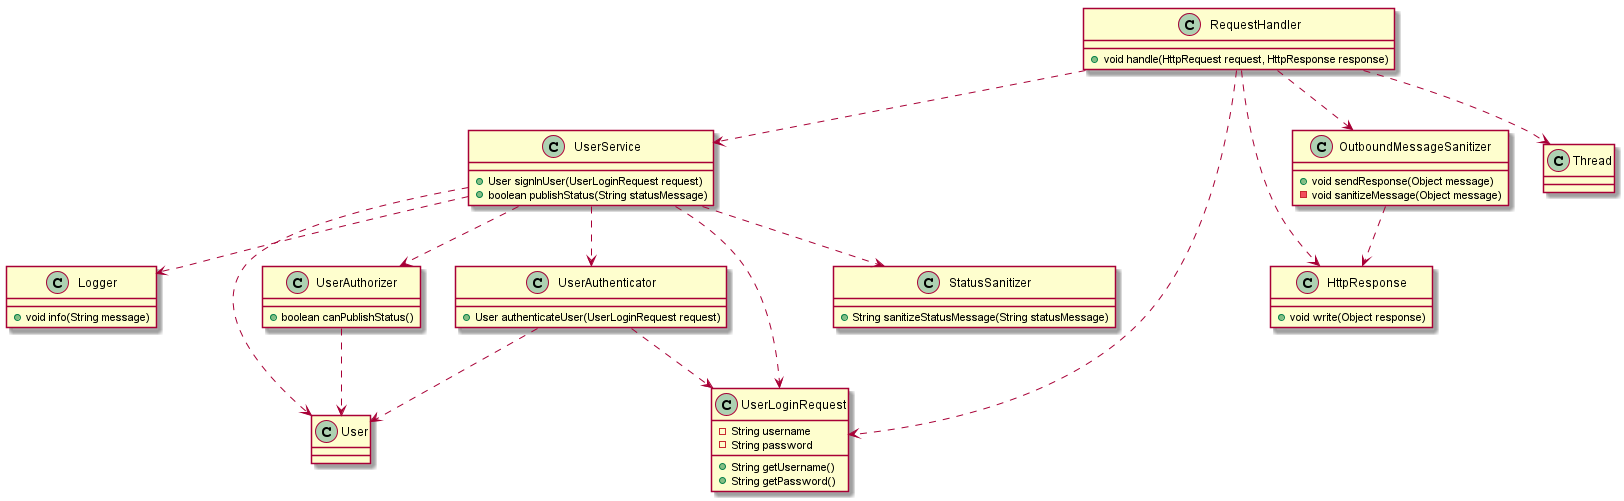
\includegraphics[width=\textwidth]{figure/ToyApp.png}
    \caption{An example of a system, for the purpose of illustrating how the constraints are applied.}
    \label{fig:toy_application}
\end{figure}

\subsection{Enforce AuthN/AuthZ at single point}
% Description
The second constraint is defined in terms of two concepts: an authentication point and an authentication enforcer. Authentication is performed through a method call to the authentication enforcer, which is a class whose sole responsibility is to authenticate an actor. This call should occur at the authentication point, and at no other points in the system, for the sake of ensuring a uniform authentication mechanism throughout the system. Authorization is enforced in the same manner, with the concepts of an authorization point and an authorization enforcer.

% Rule definition
The definition of the second constraint is detailed in Listing~\ref{lst:constraint_2_impl}. The constraint is defined as two separate rules, for the sake of clarity, but their implementations are identical.

\begin{minipage}{\linewidth}
\begin{lstlisting}[caption={Rule definition for constraint 2.}, captionpos=b, label=lst:constraint_2_impl, numbers=left]
ArchRule enforceAuthenticationAtCentralPoint(
        Class<?> authenticationPoint,
        Class<?> authenticator) {
    return CompositeArchRule.of(
        theClass(authenticationPoint)
            .should(callMethod(declaredIn(authenticator)))
    ).and(
        methods()
            .that().areDeclaredIn(authenticator)
            .should(onlyBeAccessedBy(authenticationPoint))
    );
}

ArchRule enforceAuthorizationAtCentralPoint(
        Class<?> authorizationPoint,
        Class<?> authorizer) {
    return enforceAuthenticationAtCentralPoint(
        authorizationPoint,
        authorizer
    );
}
\end{lstlisting}
\end{minipage}

% Applied to toy app
In the example system, the authentication and authorization points are both situated in the \texttt{UserService} class while authentication and authorization are enforced by the classes \texttt{UserAuthenticator} and \texttt{UserAuthorizer} respectively. The application of the rule can be seen in Listing~\ref{lst:constraint_2_toy}.

\begin{minipage}{\linewidth}
\begin{lstlisting}[caption={Application of constraint 2 to the example system.}, captionpos=b, label=lst:constraint_2_toy, numbers=left]
@ArchTest
ArchRule enforceAuthentication = SecArchUnit
    .enforceAuthenticationAtCentralPoint(UserService.class, UserAuthenticator.class);

@ArchTest
ArchRule enforceAuthorization = SecArchUnit
    .enforceAuthorizationAtCentralPoint(UserService.class, UserAuthorizer.class);
\end{lstlisting}
\end{minipage}

\subsection{Messages are sent from a central point}
...

\begin{minipage}{\linewidth}
\begin{lstlisting}[caption={Rule definition for constraint 3.}, captionpos=b, label=lst:constraint_3_impl, numbers=left]
ArchRule sendOutboundMessagesFromCentralPoint(
        Class<?> sendingPoint,
        DescribedPredicate<? super JavaClass> senderDescriptor) {
    return methods()
        .that().areDeclaredInClassesThat(senderDescriptor)
        .and(haveAtLeastOneParameter)
        .should(onlyBeAccessedBy(sendingPoint));
}
\end{lstlisting}
\end{minipage}

\section{With Additional Information in Code}

Some of the architectural constraints require that the developer injects additional information into the source code.

In some cases, this information is simply an indicator that says something about an entire class. Naming the class with a specific suffix is one approach to accomplish this. Another approach is to implement an empty interface, which is the technique used with Java's \texttt{Serializable}\footnote{https://docs.oracle.com/javase/7/docs/api/java/io/Serializable.html} interface. 

In other cases, however, the information may be required for methods of arbitrary signatures and even specific fields. For the purposes of flexibility and minimal obtrusiveness, any extra information is expressed in the form of annotations. These can be applied to classes, fields, methods and parameters without changing the underlying architecture of the system.

\todo{Specific example that requires additional information}

\todo{Show rule definition for each constraint}
\todo{Show how each constraint is used in our toy app}

\subsection{Validate user input}
...

\begin{minipage}{\linewidth}
\begin{lstlisting}[caption={Rule definition for constraint 4.}, captionpos=b, label=lst:constraint_4_impl, numbers=left]
public static ArchRule validateUserInput() {
    return codeUnits()
        .that().areAnnotatedWith(UserInput.class)
        .should(performDirectOrIndirectValidation);
}
\end{lstlisting}
\end{minipage}

\subsection{Restrict thread spawning}
While resources is a broad term, this constraint focuses on preventing the exhaustion of CPU and memory resources through the creation of new threads and processes. As such, every block of code that contains a call to the \texttt{start()} method of a \texttt{Thread}\footnote{https://docs.oracle.com/javase/7/docs/api/java/lang/Thread.html} or any of its subclasses, must be marked as containing a resource restriction mechanism. The same rule is applied for calls to \texttt{ProcessBuilder.start()}\footnote{https://docs.oracle.com/javase/7/docs/api/java/lang/Process.html} and \texttt{Runtime.exec()}\footnotemark[3], which lead to the creation of new processes.
% TODO manual footnote, adjust as necessary

The marking is done with the help of an annotation, either on the relevant method or the entire class. The decision of how the restriction mechanism is implemented is left to the developer of the system.

\begin{minipage}{\linewidth}
\begin{lstlisting}[caption={Rule definition for constraint 5.}, captionpos=b, label=lst:constraint_5_impl, numbers=left]
public static ArchRule limitResourceAllocation() {
    return noClasses()
        .that().areNotAnnotatedWith(ResourceRestriction.class)
        .should().callMethodWhere(
            aThreadIsStartedWithoutRestriction
        ).orShould().callMethodWhere(
            aProcessIsStartedWithoutRestriction
        );
}
\end{lstlisting}
\end{minipage}

\section{With Extensions to ArchUnit}

In the current ArchUnit API, a rule that aims to constrain access to a method (or field) must be expressed in terms of the type signatures of the source and target methods. Some of our constraints require knowledge about the type signature of the object that is being passed as a parameter. This is a non-issue when fields and method parameters are of the same types as the objects being passed to them. However, in cases where a method signature accepts a "more general" type, such as an \texttt{Object}, there is no way for ArchUnit to constrain the types of the objects that are actually being passed as arguments.

ArchUnit builds its representation of the architecture using ASM\footnote{\url{https://asm.ow2.io/}}, a Java bytecode analysis framework. This framework contains functionality for keeping track of the stack and local variables while analyzing the instructions of a method. With knowledge of the type signatures of the references on the stack at the time of a method call or field assignment, it is possible to determine the type signatures of objects passed as method arguments or an object being assigned to a field. Our extension provides this additional information in ArchUnit's representation of accesses to fields and methods, which the rule definitions can then make use of.

\todo{Specific example that requires an extension}

\subsection{Extensions}

\todo{Detail the extensions we made}

\subsection{Constraints}

\todo{Show rule definition for each constraint}
\todo{Show how each constraint is used in our toy app}

\subsubsection*{Do not allow sensitive information to bleed to other components}
...

\subsubsection*{Do not log secrets}
...
